\documentclass[12pt,letterpaper]{article}
\usepackage{preamble}

%%%%%%%%%%%%%%%%%%%%%%%%%%%%%%%%%%%%%%%%%%
%%%% Edit These for yourself
%%%%%%%%%%%%%%%%%%%%%%%%%%%%%%%%%%%%%%%%%%
\newcommand\course{AOE 5944 - UQML}
\newcommand\hwnumber{1}
\newcommand\userID{Kristopher Olshefski}


% Default fixed font does not support bold face
\DeclareFixedFont{\ttb}{T1}{txtt}{bx}{n}{12} % for bold
\DeclareFixedFont{\ttm}{T1}{txtt}{m}{n}{12}  % for normal

% Custom colors
\usepackage{color}
\definecolor{deepblue}{rgb}{0,0,0.5}
\definecolor{deepred}{rgb}{0.6,0,0}
\definecolor{deepgreen}{rgb}{0,0.5,0}

\usepackage{listings}

% Python style for highlighting
\newcommand\pythonstyle{\lstset{
language=Python,
basicstyle=\ttm,
otherkeywords={self},             % Add keywords here
keywordstyle=\ttb\color{deepblue},
emph={MyClass,__init__},          % Custom highlighting
emphstyle=\ttb\color{deepred},    % Custom highlighting style
stringstyle=\color{deepgreen},
frame=tb,                         % Any extra options here
showstringspaces=false            % 
}}


% Python environment
\lstnewenvironment{python}[1][]
{
\pythonstyle
\lstset{#1}
}
{}

% Python for external files
\newcommand\pythonexternal[2][]{{
\pythonstyle
\lstinputlisting[#1]{#2}}}

% Python for inline
\newcommand\pythoninline[1]{{\pythonstyle\lstinline!#1!}}




\begin{document}

    
\begin{center}
    \textbf{\Large Python \& \LaTeX}
\end{center}
\section*{Problem Description}
The problem being solved is that of temperature distribution on a two-dimensional plate which can be described by the following equation:
\begin{equation}
    (\frac{\partial u}{\partial t}=\nabla^{2} u \quad) or (\quad \frac{\partial u}{\partial t}=\frac{\partial^{2} u}{\partial x^{2}}+\frac{\partial^{2} u}{\partial y^{2}})
\end{equation}
$$    
\begin{array}{ll}
{\text { on }} & {\Omega=\left[-\frac{L_{x}}{2}, \frac{L_{x}}{2}\right] \times\left[-\frac{L_{y}}{2}, \frac{L_{y}}{2}\right]} \\
{\text { with }} & {u(t=0, x, y)=u_{0}(x, y)}
\end{array}
$$
Additionally, we set boundary conditions to reflect an insulating boundary on all sides. 

\section*{Methods}
We use a central finite differencing scheme to discretize the governing equation and create an update equation for our parameter of interest as \begin{equation}
    (u_{i, j}^{(n+1)}=u_{i, j}^{(n)}+\Delta t\left[\frac{u_{i-1, j}^{(n)}-2 u_{i, j}^{(n)}+u_{i+1, j}^{(n)}}{\Delta x^{2}}+\frac{u_{i, j-1}^{(n)}-2 u_{i, j}^{(n)}+u_{i, j+1}^{(n)}}{\Delta y^{2}}\right])
\end{equation}
where: $\Delta t$ is time step size; $\Delta x$ and $\Delta y$ are grid spacing in x and y directions, respectively;
n indicates current time level; n+1 indicates next time level; i and j are spatial indexes. We enforce a stability criteria to ensure 
\begin{equation}
    \frac{\Delta t}{\Delta x^{2}}+\frac{\Delta t}{\Delta y^{2}} \leq \frac{1}{2}
\end{equation}
\section*{Instructions}
Use of the code is fairly straightforward. User inputs are assigned in the input file which can be seen in Appendix 2. This input file provides example for all user required inputs and allows for customization of the grid size, diffusivity constant, total number of time steps, as well as other parameters. Additional parameters may be introduced by the user as deemed necessary. 

With the initial parameters set in the input file, the user simply runs the \emph{code.py} python script with a simple terminal call of *python code.py*. This will execute the code. This execution will run the analysis, create a post-processing directory, and plot relevant images in the post-processing directory. However, prior to running the script, the user should ensure that the correct initial condition is selected from the list of initial conditions. This may either reflect a step function or infinite bar solution. These are currently the only implemented initial conditions. However, the user is welcome to introduce new conditions as they see necessary.
\section*{Verification}
For code validation and verification we choose to explore an infinite bar test case and compare to an analytic solution. The initial condition set is 
\begin{equation}
    u_{0}(x)=\left\{\begin{array}{ll}
{\frac{1}{2 \varepsilon}} & {\text { if }-\varepsilon<x<\varepsilon} \\
{0} & {\text { elsewhere }}
\end{array}\right.
\end{equation}
where $\varepsilon$ is the diffusivity constant. An analytical solution exists where the output parameter can be calculated as 
\begin{equation}
    u(t, x)=\frac{1}{\sqrt{4 \pi t}} e^{-\frac{x^{2}}{4 t}}\texttt{.}
\end{equation}
With values of $\varepsilon$ as high as $1.0$ we see resulting values which correspond to an error on the order of $10^3$. However, as our value of $\varepsilon$ converges to zero, we find that we are able to achieve resulting values within $5\%$ of the analytic solution. This test case provides piece of mind that the model is performing as expected.    

\section*{Capability}
As a demonstration of capability, we set an additional initial condition. We set an initial circular heat concentration in the middle of the domain and allow for the dissipation of the parameter through our model. The initial condition is set as 
\begin{equation}
        u_{0}(x)=\left\{\begin{array}{ll}
{1} & {\text { if } ((x)\Delta x - 50)^2 + ((y)\Delta  - 50)^2<= 5} \\
{0} & {\text { elsewhere }}
\end{array}\right.
\end{equation}
This initial condition can be seen in Figure~\ref{fig:init}. 
\begin{figure}[h!]
        \centering
        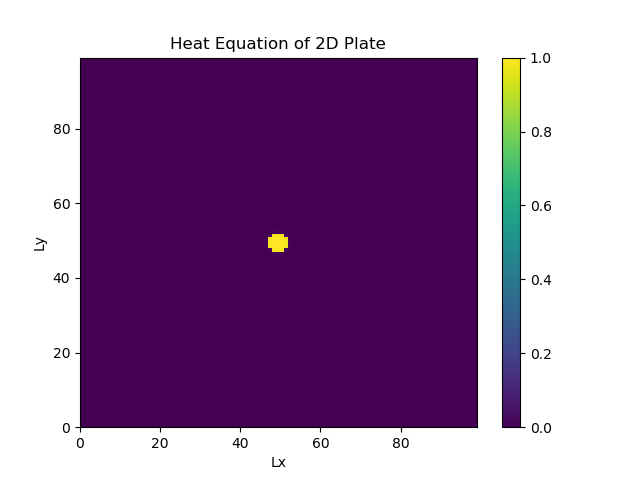
\includegraphics[scale = 0.5]{figs/init.png}
        \caption{Initial state of circular heat source}
        \label{fig:init}
\end{figure}
After $10000$ iterations the resulting temperature distribution looks as expected. The final state can be seen in Figure~\ref{fig:final}.
\begin{figure}[h!]
        \centering
        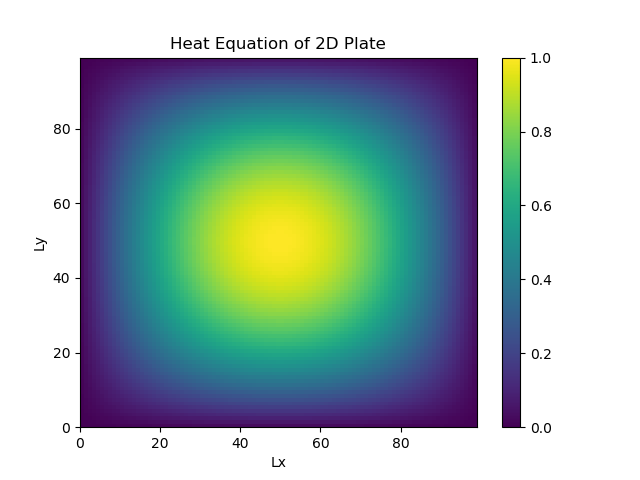
\includegraphics[scale = 0.5]{figs/final.png}
        \caption{Initial state of circular heat source}
        \label{fig:final}
\end{figure}


\section*{Closing Remarks}
This documents serves to supplement a code which is written to solve a two-dimensional heat equation. Appendix 1 \& 2 provide documentation of the code as well as the input file. 


\newpage
\section*{Appendix 1 - Code}
\pythonexternal{code/code.py}
\newpage
\section*{Appendix 2 - Input File}
\pythonexternal{code/input.py}

\end{document}
